\documentclass[a4paper,11pt]{article}

\usepackage[utf8]{inputenc}
\usepackage[T1]{fontenc}
\usepackage{amsmath,amssymb}
\usepackage{geometry}
\usepackage{hyperref}
\usepackage{graphicx}
\usepackage{tikz}
\usetikzlibrary{arrows.meta,positioning}

\geometry{margin=2.2cm}
\hypersetup{
  colorlinks=true,
  linkcolor=blue,
  urlcolor=blue
}

\title{DataLab Software Framework and Module Overview}
\author{}
\date{}

\begin{document}
\maketitle

\section{Overall Design}

DataLab targets high-precision numerical data processing and provides Extrapolation, Uncertainty Propagation, Fitting, and Statistics. The implementation follows a layered structure: an interactive UI layer + a shared core computation layer + a formatting/reporting layer. The desktop app (PySide6) and the Web app (Flask) share the same core computation and the same expression parser/function whitelist, ensuring consistent numerical results, error messages, and supported-function hints across entry points.

\subsection{System architecture breakdown}

\begin{figure}[htbp]
  \centering
  \footnotesize
  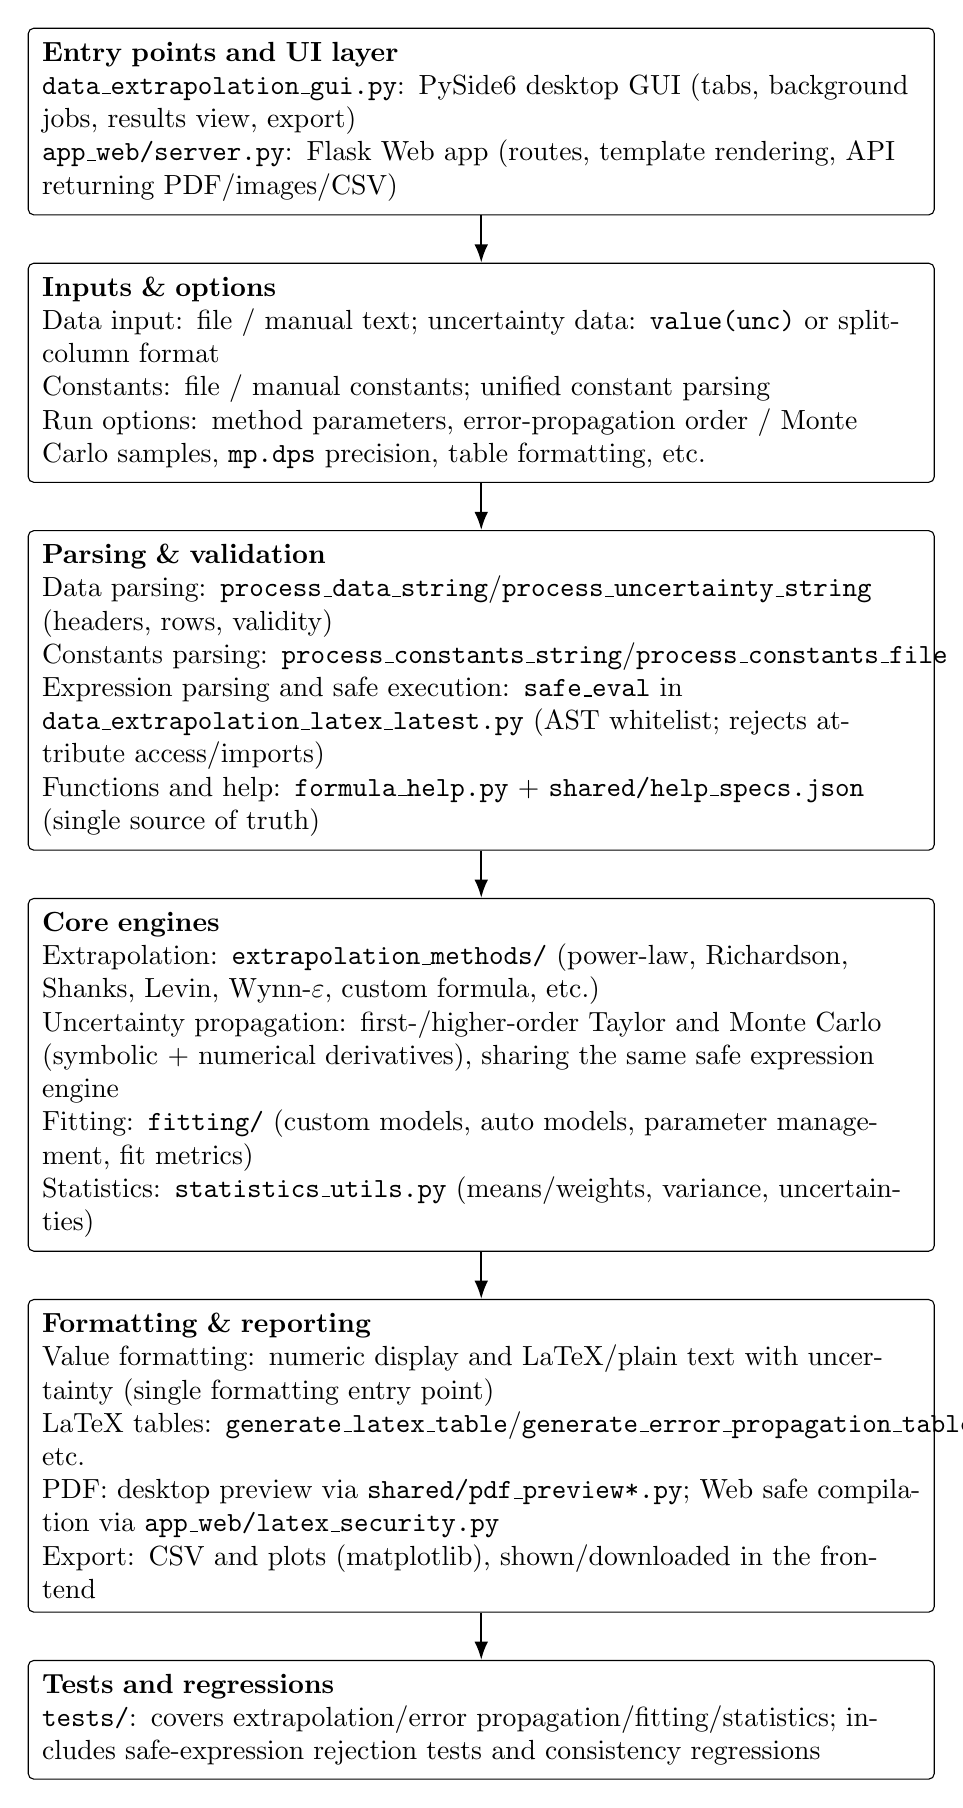
\begin{tikzpicture}[
      node distance=6mm,
      block/.style={
          rectangle,
          draw,
          rounded corners=2pt,
          align=left,
          text width=0.92\textwidth,
          inner sep=5pt
        },
      arrow/.style={-Latex, thick}
    ]
    \node[block] (entry) {\textbf{Entry points and UI layer}\\
      \texttt{data\_extrapolation\_gui.py}: PySide6 desktop GUI (tabs, background jobs, results view, export)\\
      \texttt{app\_web/server.py}: Flask Web app (routes, template rendering, API returning PDF/images/CSV)};

    \node[block, below=of entry] (input) {\textbf{Inputs \& options}\\
      Data input: file / manual text; uncertainty data: \texttt{value(unc)} or split-column format\\
      Constants: file / manual constants; unified constant parsing\\
      Run options: method parameters, error-propagation order / Monte Carlo samples, \texttt{mp.dps} precision, table formatting, etc.};
    \draw[arrow] (entry) -- (input);

    \node[block, below=of input] (parse) {\textbf{Parsing \& validation}\\
      Data parsing: \texttt{process\_data\_string}/\texttt{process\_uncertainty\_string} (headers, rows, validity)\\
      Constants parsing: \texttt{process\_constants\_string}/\texttt{process\_constants\_file}\\
      Expression parsing and safe execution: \texttt{safe\_eval} in \texttt{data\_extrapolation\_latex\_latest.py} (AST whitelist; rejects attribute access/imports)\\
      Functions and help: \texttt{formula\_help.py} + \texttt{shared/help\_specs.json} (single source of truth)};
    \draw[arrow] (input) -- (parse);

    \node[block, below=of parse] (engine) {\textbf{Core engines}\\
      Extrapolation: \texttt{extrapolation\_methods/} (power-law, Richardson, Shanks, Levin, Wynn-$\varepsilon$, custom formula, etc.)\\
      Uncertainty propagation: first-/higher-order Taylor and Monte Carlo (symbolic + numerical derivatives), sharing the same safe expression engine\\
      Fitting: \texttt{fitting/} (custom models, auto models, parameter management, fit metrics)\\
      Statistics: \texttt{statistics\_utils.py} (means/weights, variance, uncertainties)};
    \draw[arrow] (parse) -- (engine);

    \node[block, below=of engine] (output) {\textbf{Formatting \& reporting}\\
      Value formatting: numeric display and LaTeX/plain text with uncertainty (single formatting entry point)\\
      LaTeX tables: \texttt{generate\_latex\_table}/\texttt{generate\_error\_propagation\_table}, etc.\\
      PDF: desktop preview via \texttt{shared/pdf\_preview*.py}; Web safe compilation via \texttt{app\_web/latex\_security.py}\\
      Export: CSV and plots (matplotlib), shown/downloaded in the frontend};
    \draw[arrow] (engine) -- (output);

    \node[block, below=of output] (tests) {\textbf{Tests and regressions}\\
      \texttt{tests/}: covers extrapolation/error propagation/fitting/statistics; includes safe-expression rejection tests and consistency regressions};
    \draw[arrow] (output) -- (tests);
  \end{tikzpicture}
  \caption{DataLab source code architecture and major module relationships (width constrained by the A4 text width)}
  \label{fig:datalab-framework}
\end{figure}

\subsection{Function and sub-function trees}

From a user workflow perspective, the four major functions (Extrapolation, Error propagation, Fitting, Statistics) share a consistent pipeline: input $\rightarrow$ configuration $\rightarrow$ execution $\rightarrow$ output/export. The differences are mainly in: Extrapolation focusing on method selection and parameters; Error propagation focusing on formula + constants + order/sampling; Fitting focusing on column selection + model/parameter configuration; Statistics focusing on column selection + batching/variance options. To avoid overcrowding, Figures~\ref{fig:datalab-function-tree-extrap}--\ref{fig:datalab-function-tree-stats} show the sub-function trees separately.

\begin{figure}[htbp]
  \centering
  \scriptsize
  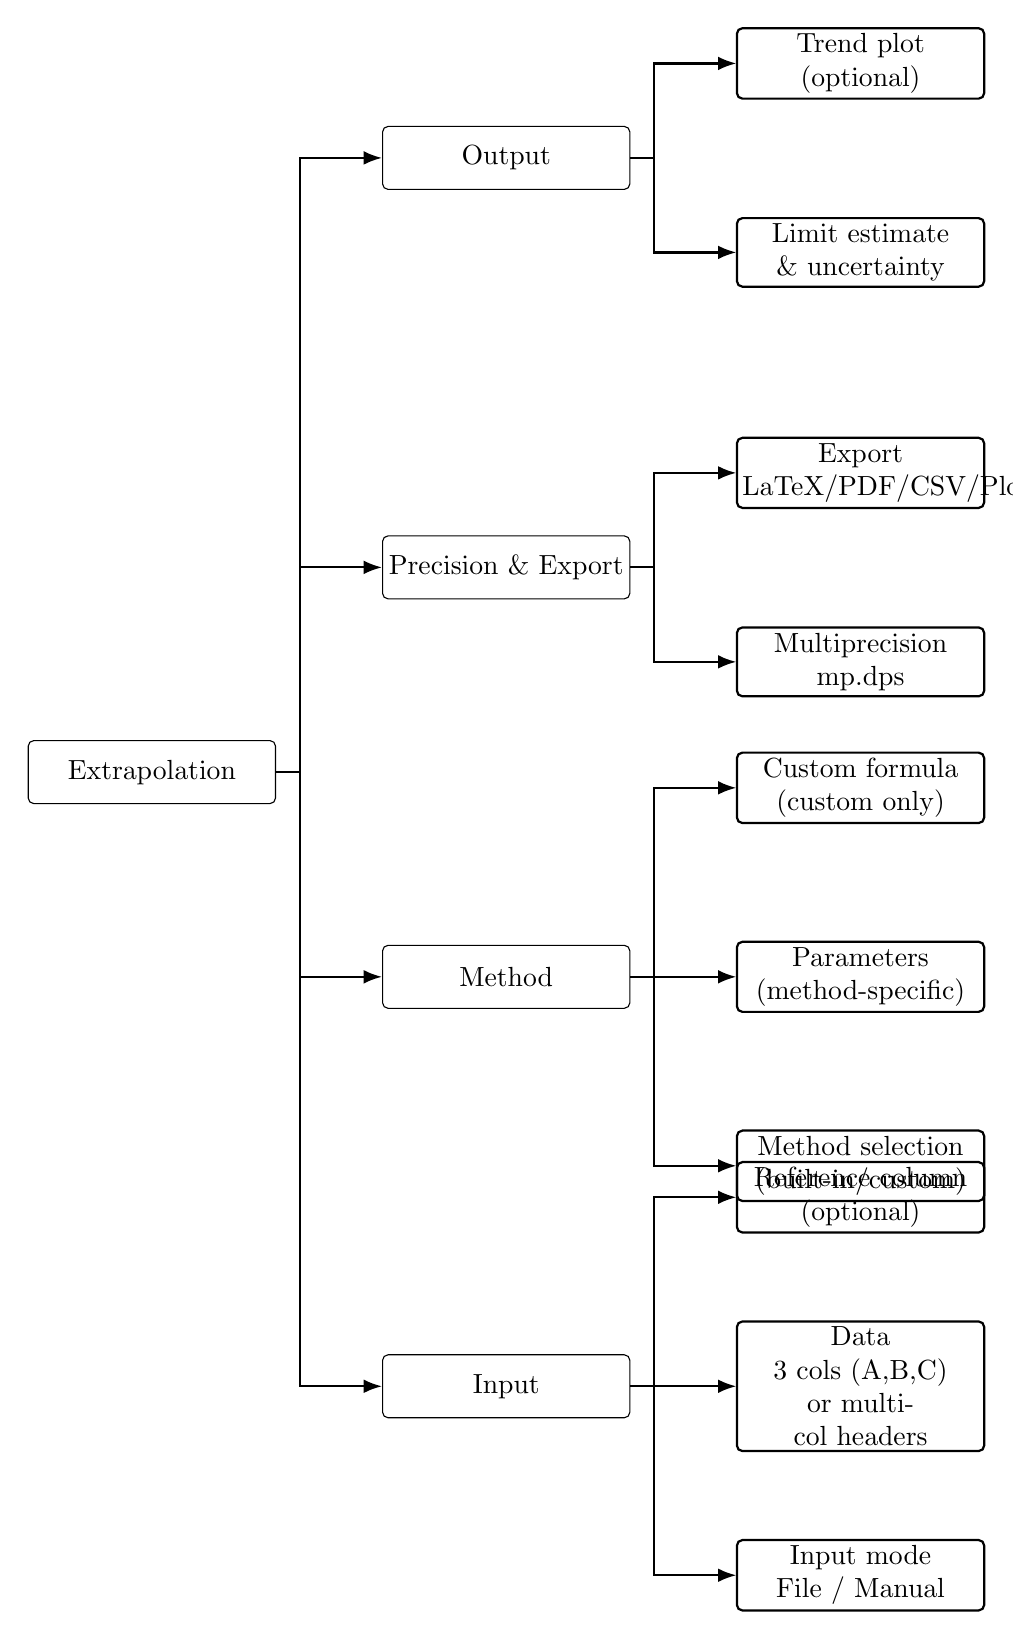
\begin{tikzpicture}[
      grow=right,
      level distance=45mm,
      edge from parent/.style={draw, -Latex, thick},
      edge from parent path={(\tikzparentnode.east) -- +(3mm,0) |- (\tikzchildnode.west)},
      box/.style={
          rectangle, draw, rounded corners=2pt,
          align=center,
          text width=3.0cm,       % previously 3.4cm; slightly narrower for layout
          inner sep=2pt,
          minimum height=8mm      % keep short labels from looking too squashed
        },
      level 1/.style={sibling distance=52mm}, % previously 44mm
      level 2/.style={sibling distance=24mm}, % previously 18mm
      level 3/.style={sibling distance=14mm}, % previously 10mm
    ]
    \node[box]{Extrapolation}
    child { node[box]{Input}
        child { node[box]{Input mode\\File / Manual} }
        child { node[box]{Data\\3 cols (A,B,C)\\or multi-col headers} }
        child { node[box]{Reference column\\(optional)} }
      }
    child { node[box]{Method}
        child { node[box]{Method selection\\(built-in/custom)} }
        child { node[box]{Parameters\\(method-specific)} }
        child { node[box]{Custom formula\\(custom only)} }
      }
    child { node[box]{Precision \& Export}
        child { node[box]{Multiprecision\\mp.dps} }
        child { node[box]{Export\\LaTeX/PDF/CSV/Plots} }
      }
    child { node[box]{Output}
        child { node[box]{Limit estimate\\\& uncertainty} }
        child { node[box]{Trend plot\\(optional)} }
      };
  \end{tikzpicture}
  \caption{Sub-function tree of the extrapolation module}
  \label{fig:datalab-function-tree-extrap}
\end{figure}

\begin{figure}[htbp]
  \centering
  \scriptsize
  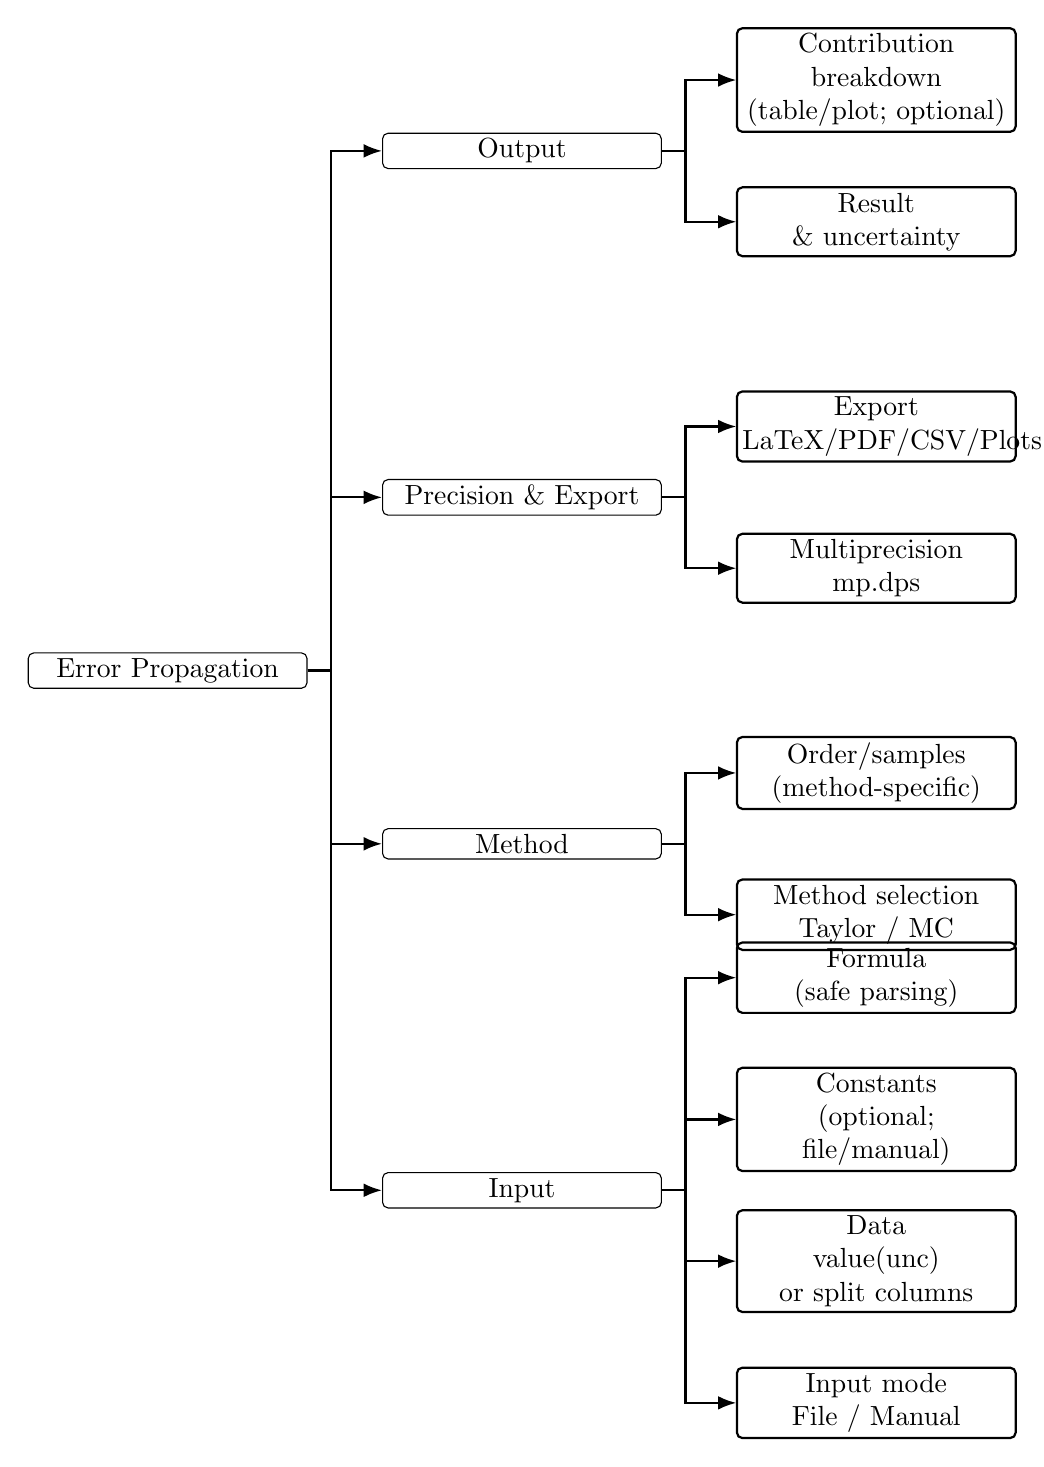
\begin{tikzpicture}[
      grow=right,
      level distance=45mm,
      edge from parent/.style={draw, -Latex, thick},
      edge from parent path={(\tikzparentnode.east) -- +(3mm,0) |- (\tikzchildnode.west)},
      box/.style={rectangle, draw, rounded corners=2pt, align=center, text width=3.4cm, inner sep=2pt},
      level 1/.style={sibling distance=44mm},
      level 2/.style={sibling distance=18mm},
      level 3/.style={sibling distance=10mm},
    ]
    \node[box]{Error Propagation}
    child { node[box]{Input}
        child { node[box]{Input mode\\File / Manual} }
        child { node[box]{Data\\value(unc)\\or split columns} }
        child { node[box]{Constants\\(optional; file/manual)} }
        child { node[box]{Formula\\(safe parsing)} }
      }
    child { node[box]{Method}
        child { node[box]{Method selection\\Taylor / MC} }
        child { node[box]{Order/samples\\(method-specific)} }
      }
    child { node[box]{Precision \& Export}
        child { node[box]{Multiprecision\\mp.dps} }
        child { node[box]{Export\\LaTeX/PDF/CSV/Plots} }
      }
    child { node[box]{Output}
        child { node[box]{Result\\\& uncertainty} }
        child { node[box]{Contribution breakdown\\(table/plot; optional)} }
      };
  \end{tikzpicture}
  \caption{Sub-function tree of the error propagation module}
  \label{fig:datalab-function-tree-error}
\end{figure}

\begin{figure}[htbp]
  \centering
  \scriptsize
  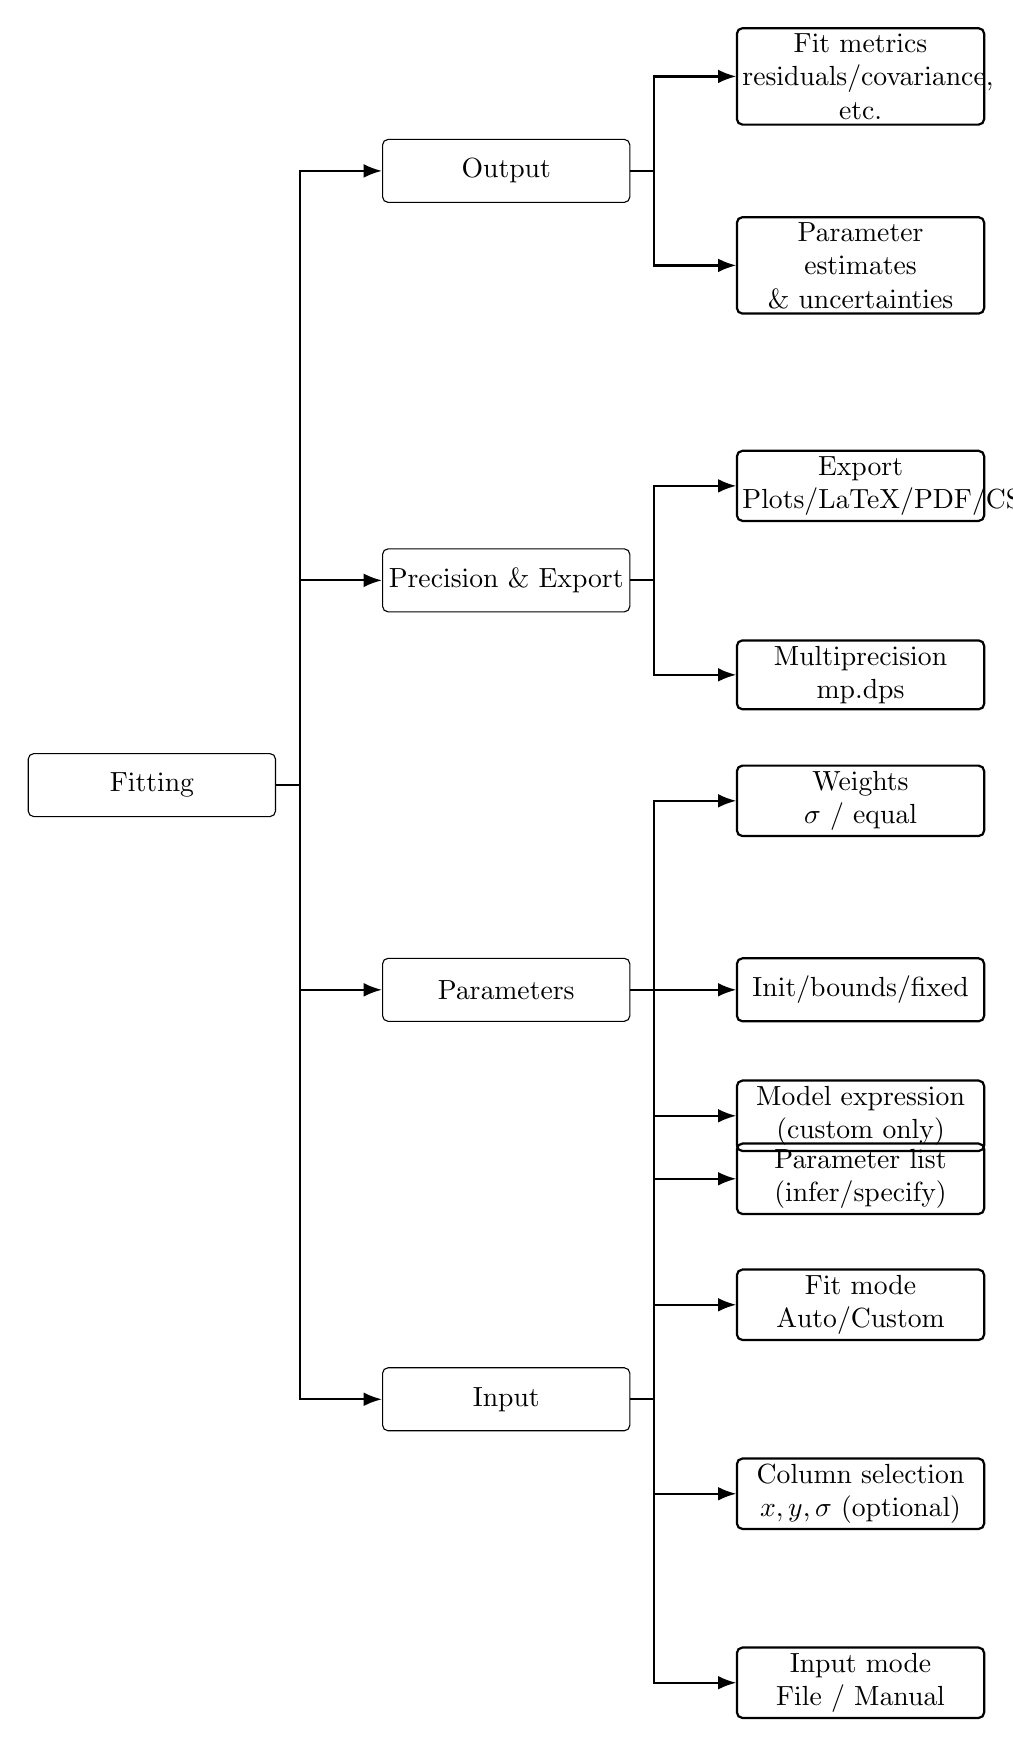
\begin{tikzpicture}[
      grow=right,
      level distance=45mm,
      edge from parent/.style={draw, -Latex, thick},
      edge from parent path={(\tikzparentnode.east) -- +(3mm,0) |- (\tikzchildnode.west)},
      box/.style={
          rectangle, draw, rounded corners=2pt,
          align=center,
          text width=3.0cm,       % previously 3.4cm; slightly narrower for layout
          inner sep=2pt,
          minimum height=8mm
        },
      level 1/.style={sibling distance=52mm},
      level 2/.style={sibling distance=24mm},
      level 3/.style={sibling distance=14mm},
    ]
    \node[box]{Fitting}
    child { node[box]{Input}
        child { node[box]{Input mode\\File / Manual} }
        child { node[box]{Column selection\\$x,y,\sigma$ (optional)} }
        child { node[box]{Fit mode\\Auto/Custom} }
        child { node[box]{Model expression\\(custom only)} }
      }
    child { node[box]{Parameters}
        child { node[box]{Parameter list\\(infer/specify)} }
        child { node[box]{Init/bounds/fixed} }
        child { node[box]{Weights\\$\sigma$ / equal} }
      }
    child { node[box]{Precision \& Export}
        child { node[box]{Multiprecision\\mp.dps} }
        child { node[box]{Export\\Plots/LaTeX/PDF/CSV} }
      }
    child { node[box]{Output}
        child { node[box]{Parameter estimates\\\& uncertainties} }
        child { node[box]{Fit metrics\\residuals/covariance, etc.} }
      };
  \end{tikzpicture}
  \caption{Sub-function tree of the fitting module}
  \label{fig:datalab-function-tree-fit}
\end{figure}

\begin{figure}[htbp]
  \centering
  \scriptsize
  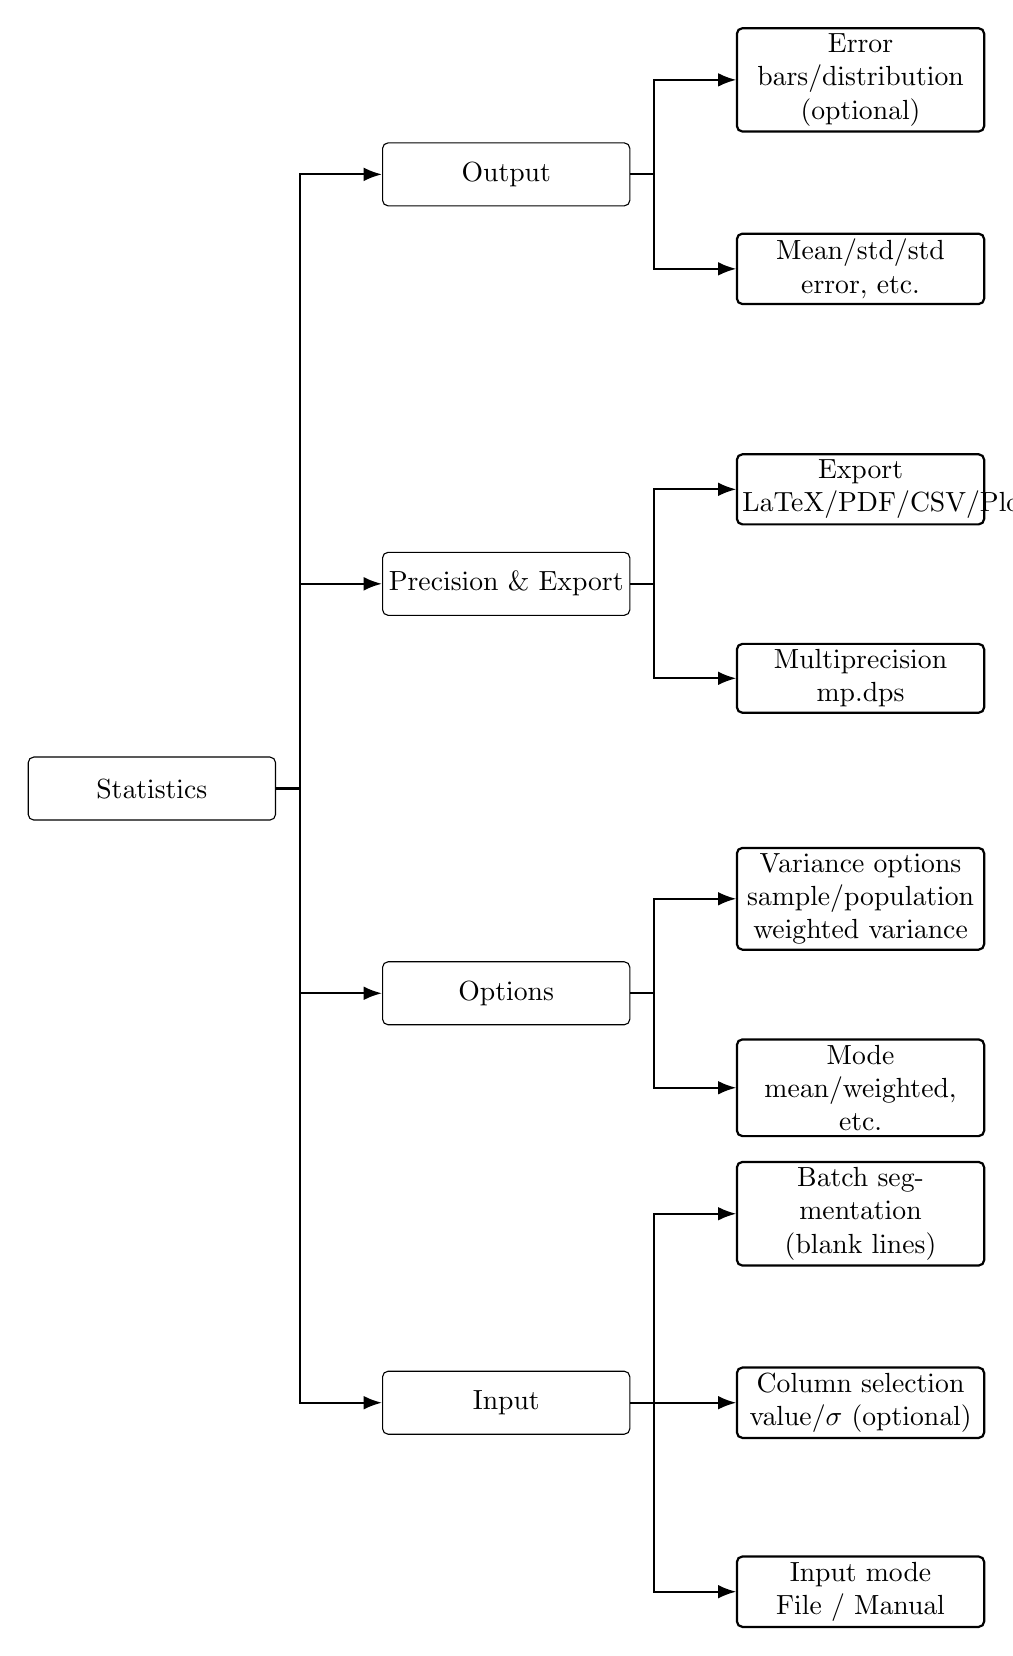
\begin{tikzpicture}[
      grow=right,
      level distance=45mm,
      edge from parent/.style={draw, -Latex, thick},
      edge from parent path={(\tikzparentnode.east) -- +(3mm,0) |- (\tikzchildnode.west)},
      box/.style={
          rectangle, draw, rounded corners=2pt,
          align=center,
          text width=3.0cm,       % previously 3.4cm; slightly narrower for layout
          inner sep=2pt,
          minimum height=8mm
        },
      level 1/.style={sibling distance=52mm},
      level 2/.style={sibling distance=24mm},
      level 3/.style={sibling distance=14mm},
    ]
    \node[box]{Statistics}
    child { node[box]{Input}
        child { node[box]{Input mode\\File / Manual} }
        child { node[box]{Column selection\\value/$\sigma$ (optional)} }
        child { node[box]{Batch segmentation\\(blank lines)} }
      }
    child { node[box]{Options}
        child { node[box]{Mode\\mean/weighted, etc.} }
        child { node[box]{Variance options\\sample/population\\weighted variance} }
      }
    child { node[box]{Precision \& Export}
        child { node[box]{Multiprecision\\mp.dps} }
        child { node[box]{Export\\LaTeX/PDF/CSV/Plots} }
      }
    child { node[box]{Output}
        child { node[box]{Mean/std/std error, etc.} }
        child { node[box]{Error bars/distribution\\(optional)} }
      };
  \end{tikzpicture}
  \caption{Sub-function tree of the statistics module}
  \label{fig:datalab-function-tree-stats}
\end{figure}

\subsection{Module responsibilities}

\subsubsection{Entry points and UI layer}
The desktop and Web entry points serve different scenarios: the desktop app focuses on interactive processing, browsing results, and local PDF preview; the Web app focuses on lightweight deployment, cross-platform access, and online export. Neither UI implements algorithm details directly. Instead, both are responsible for:
\begin{itemize}
  \item collecting user inputs (data/constants/formulas/method parameters/precision settings) and constructing computation jobs;
  \item calling the shared core computation layer and receiving a unified result payload and warnings;
  \item presenting outputs as ``value + uncertainty + LaTeX + optional plots/files'' and supporting exports.
\end{itemize}

\subsubsection{Input and parsing layer}
The parsing layer converts text/files into structured data and performs strict validation to avoid implicit downstream errors:
\begin{itemize}
  \item table parsing: detect headers, convert rows to high-precision numbers (\texttt{mp.mpf}), and report missing columns/invalid characters/blank lines;
  \item uncertainty parsing: support both \texttt{value(unc)} notation and split-column inputs, normalizing into (nominal value, standard uncertainty);
  \item constants parsing: support file and manual inputs, building a constant namespace for expression evaluation and model fitting.
\end{itemize}

\subsubsection{Expression parsing and safe evaluation}
Custom extrapolation formulas, error-propagation formulas, and custom fitting models share the same safe expression engine. The core idea is to parse expressions with an AST and allow only whitelisted node types, function calls, and constants, while explicitly rejecting attribute access, imports, arbitrary object construction, and other dangerous behaviors. This design provides:
\begin{itemize}
  \item security: avoids code execution risks of \texttt{eval/exec};
  \item consistency: all formula inputs share the same function/constant registry and error-message style;
  \item extensibility: adding a function to the whitelist enables it across all formula-based scenarios and keeps help/hints in sync.
\end{itemize}

\subsubsection{Core engines}
The core engines implement the four classes of computations and use a unified precision control (\texttt{mp.dps}) for numerical stability:
\begin{itemize}
  \item extrapolation: multiple acceleration/extrapolation methods plus custom three-point formulas, producing a limit estimate and uncertainty;
  \item uncertainty propagation: first-order, higher-order Taylor contributions, and Monte Carlo sampling; outputs values, uncertainties, and optional contribution breakdowns;
  \item fitting: custom and auto models, producing parameter estimates, fitted curves, and metrics (e.g., covariance matrices and parameter uncertainties);
  \item statistics: batch-aware and weighted statistics, producing mean/variance/standard error and related indicators.
\end{itemize}

\subsubsection{Formatting and reporting}
The output layer formats results for readability and reuse, supporting both on-screen display and LaTeX export while keeping precision and formatting rules consistent:
\begin{itemize}
  \item uncertainty formatting: a single LaTeX/plain-text formatting entry point to avoid cross-module inconsistencies;
  \item LaTeX tables: unified table environments, numeric column specs (\texttt{dcolumn}/\texttt{siunitx}), segmentation, etc.;
  \item PDF: desktop preview and zoom; Web safe compilation (engine whitelist, shell-escape disabled, resource limits).
\end{itemize}

\subsubsection{Shared specifications and consistency guarantees}
To ensure ``same computation, same behavior'' across UIs, UI-facing specifications (supported functions, method descriptions, parameter visibility) are maintained centrally. For example, \texttt{formula\_help.py} and \texttt{shared/help\_specs.json} provide the unified function list and help text, and \texttt{shared/ui\_specs.py} describes method parameters and display rules. Frontends render these specifications rather than hardcoding function lists or duplicating specs.

\subsubsection{Tests and regressions}
The project uses \texttt{pytest} to maintain regression tests covering correctness, consistency, and security. Typical checks include cross-module consistency for representative formulas and special functions; rejection tests for dangerous expressions; and targeted unit tests with numeric tolerances for newer features (higher-order propagation, custom fitting models, etc.).

\end{document}
